\documentclass{beamer}
\usetheme{metropolis}

\usepackage{tikz,tikz-dependency}
\usetikzlibrary{shapes.geometric, arrows}
\tikzstyle{service} = [rectangle, minimum width=2cm, minimum height=1cm, text centered, draw=black, fill=white]
\tikzstyle{flow} = [thick,->,>=stealth]
\tikzstyle{depends} = [thick,-,>=stealth]

\usepackage{pifont, amssymb}
\newcommand{\cmark}{\ding{51}}
\newcommand{\xmark}{\ding{55}}

\newcommand\TBox[3][]{%
  \tikz\node[draw,thick,text width=#2,align=left,#1] {#3};}

\title{An argumentation-based approach to summarizing discussions}
\date{}
\author{Dr. Advaith Siddharthan, Dr. Adam Wyner \& Charlie Egan}
\institute{University of Aberdeen}

\begin{document}
  \maketitle
  \begin{frame}{Itinerary}
    \begin{enumerate}
      \item{Introduction}
      \item{Summary Comparison \& Feedback}
      \item{Motivations}
      \item{Extracting Points}
      \item{Generating Summaries}
      \item{Results}
      \item{Further Work}
      \item{Discussion}
	\end{enumerate}
  \end{frame}

  \begin{frame}{Summary Comparison \& Feedback}
	Compare two ~300 word summaries on the same topic.

	\vfill

	Consider their usefulness, which sections are most interesting?

	Can you think of sections that might be useful that are missing?

	\vfill

    Comments can be written on the sheets or entered at \textcolor{blue}{http://bit.ly/abdnpoints}.
  \end{frame}

  \begin{frame}{Motivations}
	\begin{center}
	  \fbox{
\includegraphics[width=0.7\textwidth]{reddit}}

	  \fbox{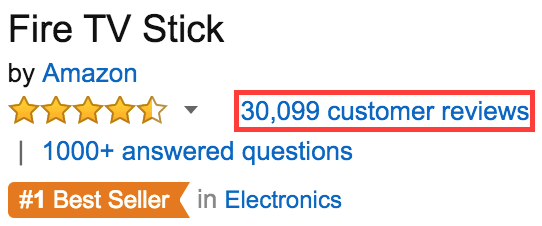
\includegraphics[width=0.5\textwidth]{fire}}

	  \fbox{
\includegraphics[width=0.6\textwidth]{tweets}}
	\end{center}
  \end{frame}

  \begin{frame}{What makes up a discussion?}
    \TBox[fill=black!15]{10.5cm}{
      \textbf{Discussion} \\[1ex]
      \small{Topic: \textit{Abortion}}
      \TBox[fill=green!5]{10.2cm}{
        \textbf{Sentence} (User A) \\[1ex]
        \small{``\textit{I think Abortion should be legal, women must have the choice.\dots}''}
      }
      \TBox[fill=red!5]{10.2cm}{
        \textbf{Sentence} (User B) \\[1ex]
        \small{``\textit{Abortion is wrong, I believe that a fetus has rights.\dots}''}
      }
      \TBox[fill=yellow!5]{10.2cm}{\dots}
	}
  \end{frame}

  \begin{frame}{Extracting Points (1/3)}
    \TBox[fill=green!5]{10.5cm}{
      \textbf{Sentence} \\[1ex]

      \small{``\textit{I think Abortion should be legal, women must have the choice.}''}

      \TBox[fill=black!15]{10.2cm}{
        Point 1 \\[1ex]
        \TBox[fill=black!5]{9.9cm}{Extract \hfill \textit{Abortion should be legal}}
        \TBox[fill=black!5]{9.9cm}{Verb \hfill be}
        \TBox[fill=black!5]{9.9cm}{
          Pattern \hfill \texttt{abortion.subject \textcolor{blue}{be.verb} legal.object}
        }
      }
      \TBox[fill=black!15]{10.2cm}{
        Point 2 \\[1ex]
        \TBox[fill=black!5]{9.9cm}{Extract \hfill \textit{women must have the choice}}
        \TBox[fill=black!5]{9.9cm}{Verb \hfill have}
        \TBox[fill=black!5]{9.9cm}{
          Pattern \hfill \texttt{women.subject \textcolor{blue}{have.verb} choice.object}
        }
      }
    }
    Point 0, ``\textit{I think}'', is also identified.
  \end{frame}

  \begin{frame}{Extracting Points (2/3)}
	\begin{itemize}
	  \item[]{\textcolor{gray}{\textbf{Extract:} ``\textit{women must have the choice}''}}
	  \item[]{\textcolor{gray}{\textbf{Verb:} have}}
	  \item[]{\textbf{Pattern:} \texttt{woman.subj \textcolor{blue}{have.verb} choice.obj}}
	\end{itemize}

	\begin{center}
	  \begin{dependency}[edge horizontal padding=0]
		\begin{deptext}
		  I \& think \& Abortion \& should \& be \& legal \&, \& women \& must \& have \& the \& choice \& . \\
		\end{deptext}
		\depedge{10}{12}{obj}
		\depedge{10}{8}{subj}
		\depedge[hide label]{10}{9}{}
		\depedge[hide label]{12}{11}{}
		\deproot[edge unit distance=2.3ex]{10}{point verb}
	  \end{dependency}

	  Lemma values (women $\rightarrow$ woman) are used in point patterns
	\end{center}
  \end{frame}

  \begin{frame}{Extracting Points (3/3)}
    Verb Case Frames define allowed point patterns.
    \vfill
    \texttt{woman.subj \textcolor{blue}{have.verb} choice.obj}
    \vfill
    \TBox[fill=red!5]{\textwidth}{
      Frame A \textcolor{red}{\xmark} e.g. ``\textit{Alice had lunch with Bob.}'' \\[1ex]
      \TBox[fill=white]{1.7cm}{NP}
      \TBox[fill=black!15]{1.7cm}{have}
      \TBox[fill=white]{1.7cm}{NP}
      \TBox[fill=white]{1.7cm}{with}
      \TBox[fill=white]{1.7cm}{NP}
    }
    \TBox[fill=red!5]{\textwidth}{
      Frame B \textcolor{red}{\xmark} e.g. ``\textit{Alice had lunch at Carluccio's}'' \\[1ex]
      \TBox[fill=white]{1.7cm}{NP}
      \TBox[fill=black!15]{1.7cm}{have}
      \TBox[fill=white]{1.7cm}{NP}
      \TBox[fill=white]{1.7cm}{at}
      \TBox[fill=white]{1.7cm}{NP}
    }
    \TBox[fill=red!5]{\textwidth}{
      Frame C \textcolor{red}{\xmark} e.g. ``\textit{\textcolor{gray}{Who's had lunch?} Alice has!}'' \\[1ex]
      \TBox[fill=white]{1.7cm}{NP}
      \TBox[fill=black!15]{1.7cm}{have}
    }
    \TBox[fill=green!5]{\textwidth}{
      Frame D \textcolor{green!70!black}{\cmark} e.g. ``\textit{Alice had lunch.}'' \\[1ex]
      \TBox[fill=white]{1.7cm}{NP}
      \TBox[fill=black!15]{1.7cm}{have}
      \TBox[fill=white]{1.7cm}{NP}
    }
  \end{frame}

  \begin{frame}{What Next?}
    \texttt{life.nsubj begin.verb\\
      have.verb abortion.dobj\\
      abortion.nsubj be.verb legal.dobj\\
      PERSON.nsubj have.verb abortion.dobj\\
      PERSON.nsubj have.verb right.dobj\\
      fetus.nsubj be.verb person.dobj\\
      woman.nsubj have.verb right.dobj\\
      PERSON.nsubj be.verb pro-choice.dobj\\
      fetus.nsubj be.verb human.dobj\\
      PERSON.nsubj be.verb abortion.dobj\\
      abortion.nsubj be.verb murder.dobj\\
      life.nsubj begin.verb at.prep conception.dobj\\
      PERSON.nsubj be.verb pregnant.dobj\\
      life.nsubj begin.verb conception.dobj\\
      take.verb life.dobj\\
      abortion.nsubj be.verb wrong.dobj\\
      have.verb child.dobj\\
      fetus.nsubj be.verb being.dobj\\
      make.verb choice.dobj}
  \end{frame}

  \begin{frame}{What Next?}
	\resizebox{\textwidth}{!}{
	  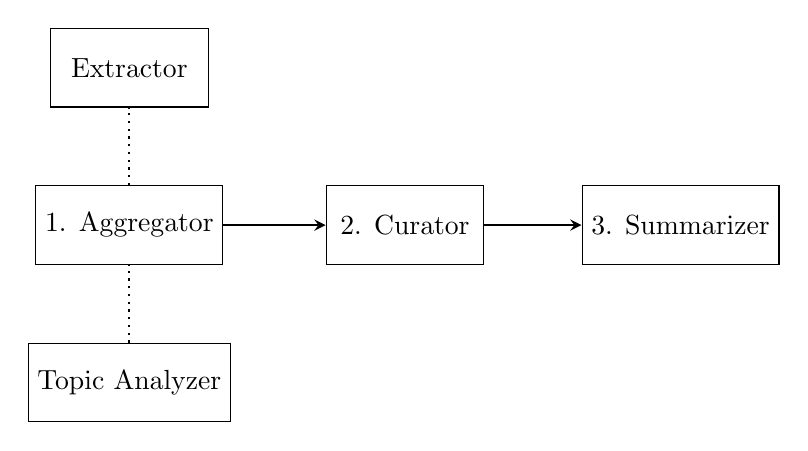
\begin{tikzpicture}[node distance=3.5cm]
		\node (agg) [service] {1. Aggregator};
		\node (top) [service, below of=agg, yshift=1.5cm] {Topic Analyzer};
		\node (ext) [service, above of=agg, yshift=-1.5cm] {Extractor};
		\node (cur) [service, right of=agg] {2. Curator};
		\node (sum) [service, right of=cur] {3. Summarizer};

		\draw [flow] (agg) -- (cur);
		\draw [flow] (cur) -- (sum);
		\draw[dotted] [depends] (agg) -- (ext);
		\draw[dotted] [depends] (top) -- (agg);
	  \end{tikzpicture}
	}
  \end{frame}

  \begin{frame}{What Next?}
    \fbox{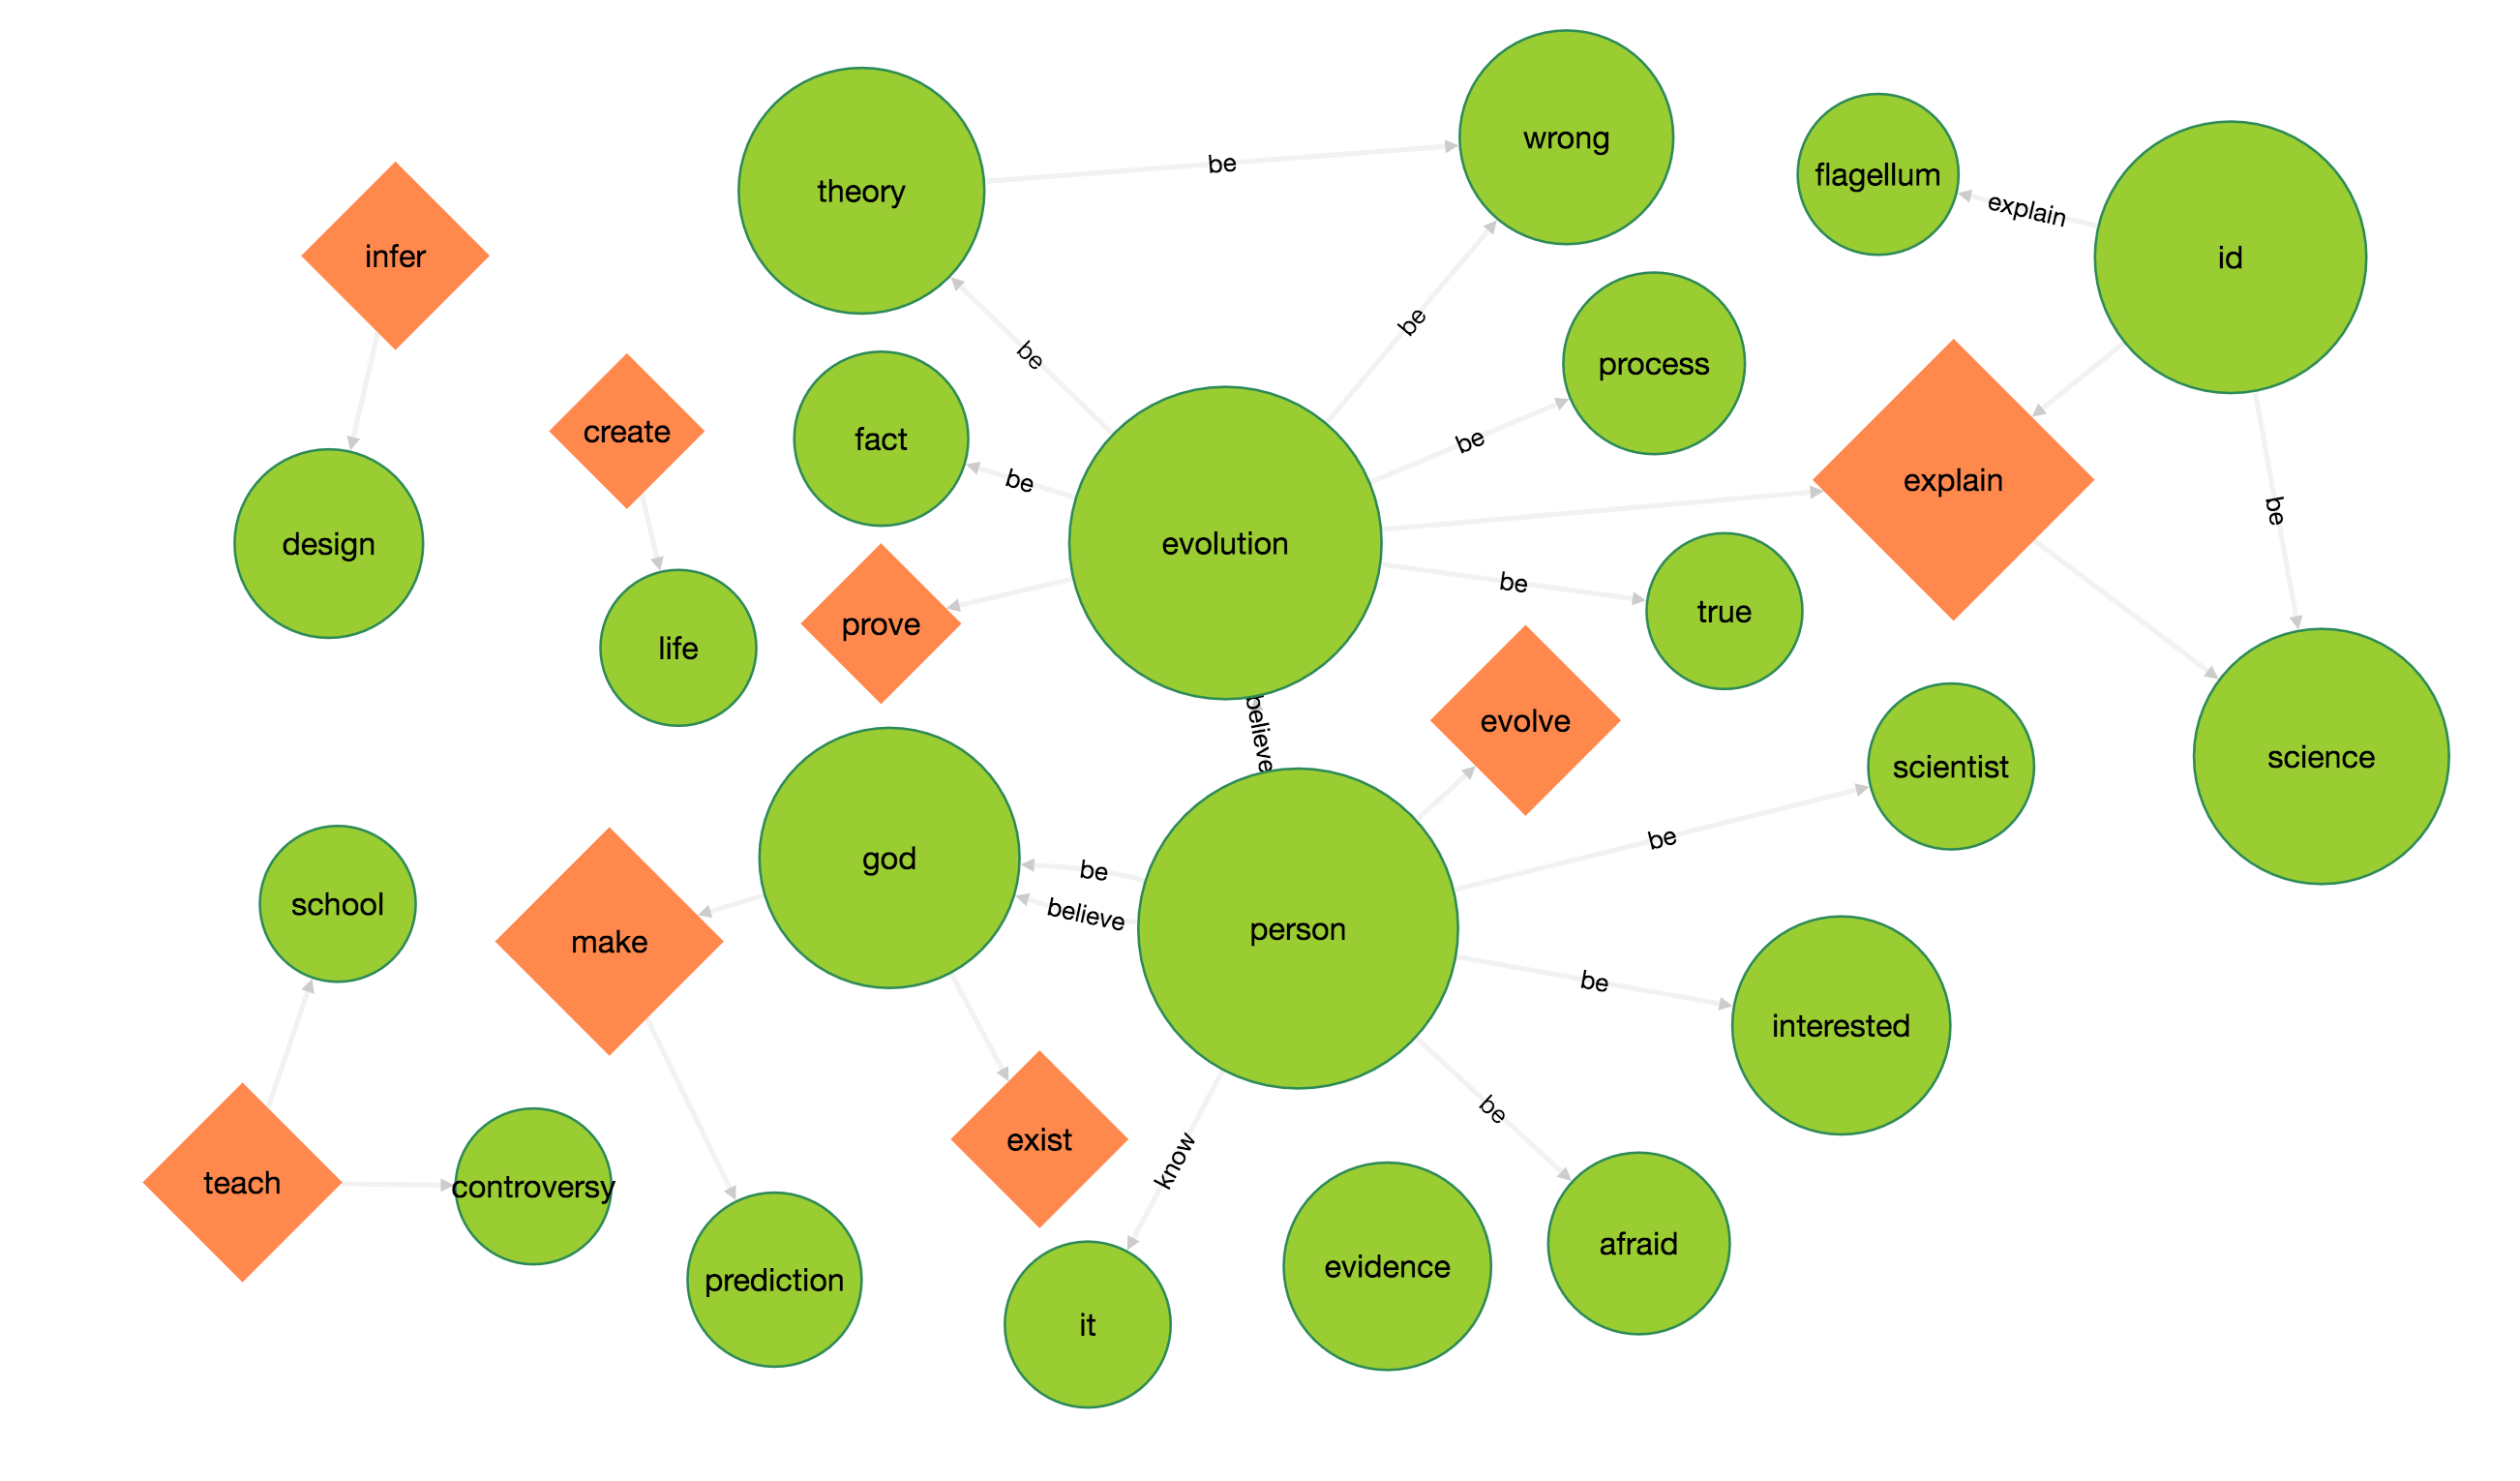
\includegraphics[width=\textwidth]{disc_graph}}
  \end{frame}

  \begin{frame}{Generating Summaries (1/4)}
    \textbf{Identifying Counter Points}

    \texttt{mother.nsubj have.verb right.dobj}\\
    \begin{center}
      using antonyms\\$\downarrow$
    \end{center}
    \texttt{\textcolor{red}{father.nsubj} have.verb right.dobj}\\
    \texttt{mother.nsubj \textcolor{red}{lack.verb} right.dobj}\\
    \texttt{mother.nsubj have.verb \textcolor{red}{left.dobj}}
  \end{frame}

  \begin{frame}{Generating Summaries (2/4)}
    \textbf{Matched Negated Points}

    \begin{center}
      ``\textit{A fetus is a human being}''
      \&
      ``\textit{A fetus is \textbf{not} a human being}''\\
      $\downarrow$ \\
      ``\textit{A fetus is \textbf{\{}not\textbf{\}} a human being}''
    \end{center}
  \end{frame}

  \begin{frame}{Generating Summaries (3/4)}
    \textbf{Related Points}
  	Discussion Model
	\vfill
	\TBox[fill=black!5]{10cm}{
	  Example Discussion \\[1ex]
	  \TBox[fill=black!10]{4.65cm}{
        Post A (User 1) \\[1ex]
		\TBox[fill=red!15]{1.17cm}{\small Point 1}
		\TBox[fill=green!35]{1.17cm}{\small Point 2}
		\TBox[fill=blue!35]{1.17cm}{\small Point 3}
	  }
	  \TBox[fill=black!10]{4.65cm}{
        Post B (User 2) \\[1ex]
		\TBox[fill=green!35]{1.17cm}{\small Point 2}
		\TBox[fill=blue!35]{1.17cm}{\small Point 3}
		\TBox[fill=yellow!15]{1.17cm}{\small Point 4}
	  }
	  \TBox[fill=black!10]{4.65cm}{
        Post C (User 3) \\[1ex]
		\TBox[fill=green!15]{1.17cm}{\small Point 2}
		\TBox[fill=yellow!15]{1.17cm}{\small Point 4}
		\TBox[fill=orange!15]{1.17cm}{\small Point 5}
	  }
	  \TBox[fill=black!10]{4.65cm}{
        Post D (User 4) \\[1ex]
		\TBox[fill=orange!15]{1.17cm}{\small Point 5}
		\TBox[fill=blue!35]{1.17cm}{\small Point 3}
		\TBox[fill=green!35]{1.17cm}{\small Point 2}
	  }
	}
	\vfill
    \TBox[fill=green!35]{1.17cm}{\small Point 2}
    \TBox[fill=blue!35]{1.17cm}{\small Point 3}\\
    Points 2 \& 3 are a common pair, raised together by 3 different posts.
  \end{frame}

  \begin{frame}{Generating Summaries (4/4)}
    \textbf{Other summary sections:}\\
    \begin{itemize}
      \item{Commonly occurring points}
      \item{Points that reference multiple topics}
      \item{Points with longer patterns}
      \item{Top points for core topics}
      \item{Questions asked}
    \end{itemize}
  \end{frame}

  \begin{frame}{Evaluation \& Results}
    Participants on Amazon Mechanical Turk compared summaries

    \fbox{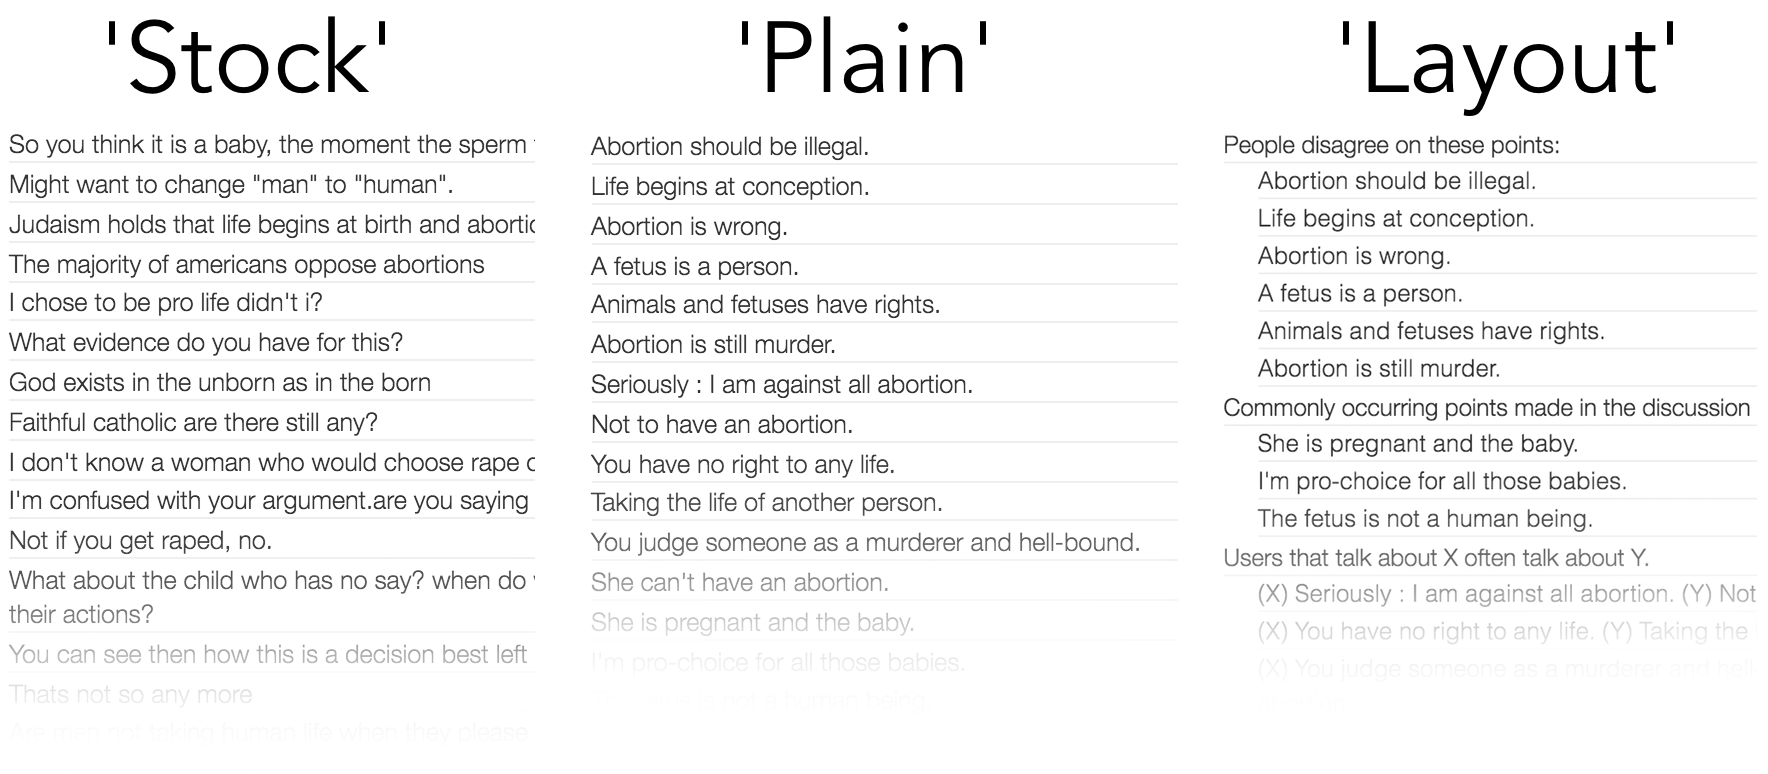
\includegraphics[width=0.95\textwidth]{summaries}}
  \end{frame}

  \begin{frame}{Evaluation \& Results}
	\begin{center}
	  \fbox{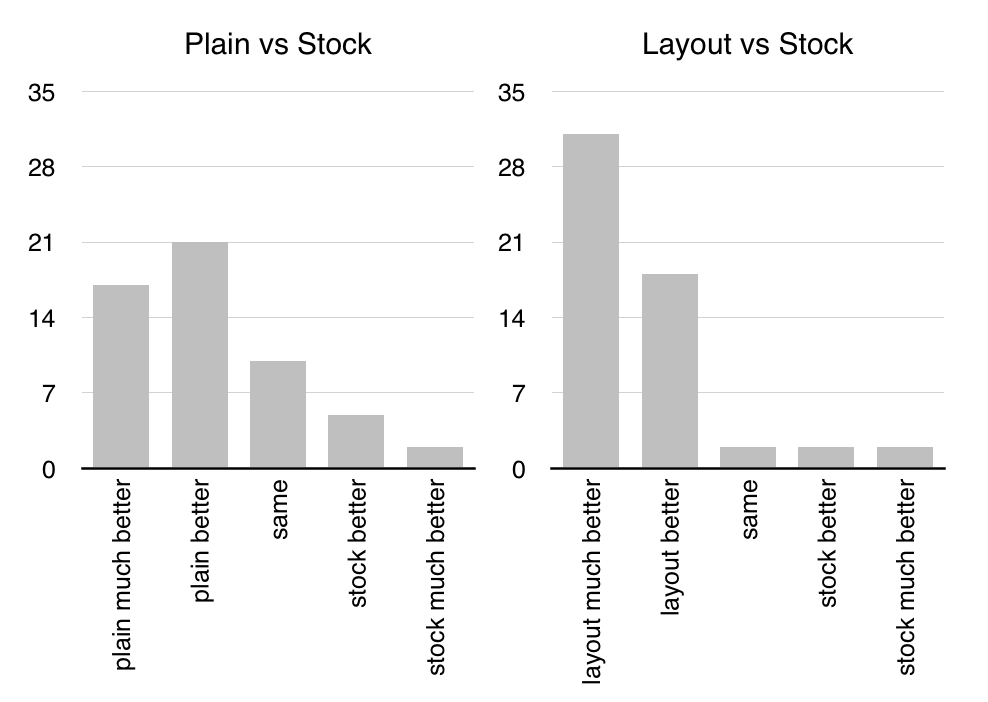
\includegraphics[width=0.85\textwidth]{results}}
	\end{center}
  \end{frame}

  \begin{frame}{Questions}
    \begin{center}
      \texttt{we.subject \textcolor{red}{have.verb} point.object}
      \fbox{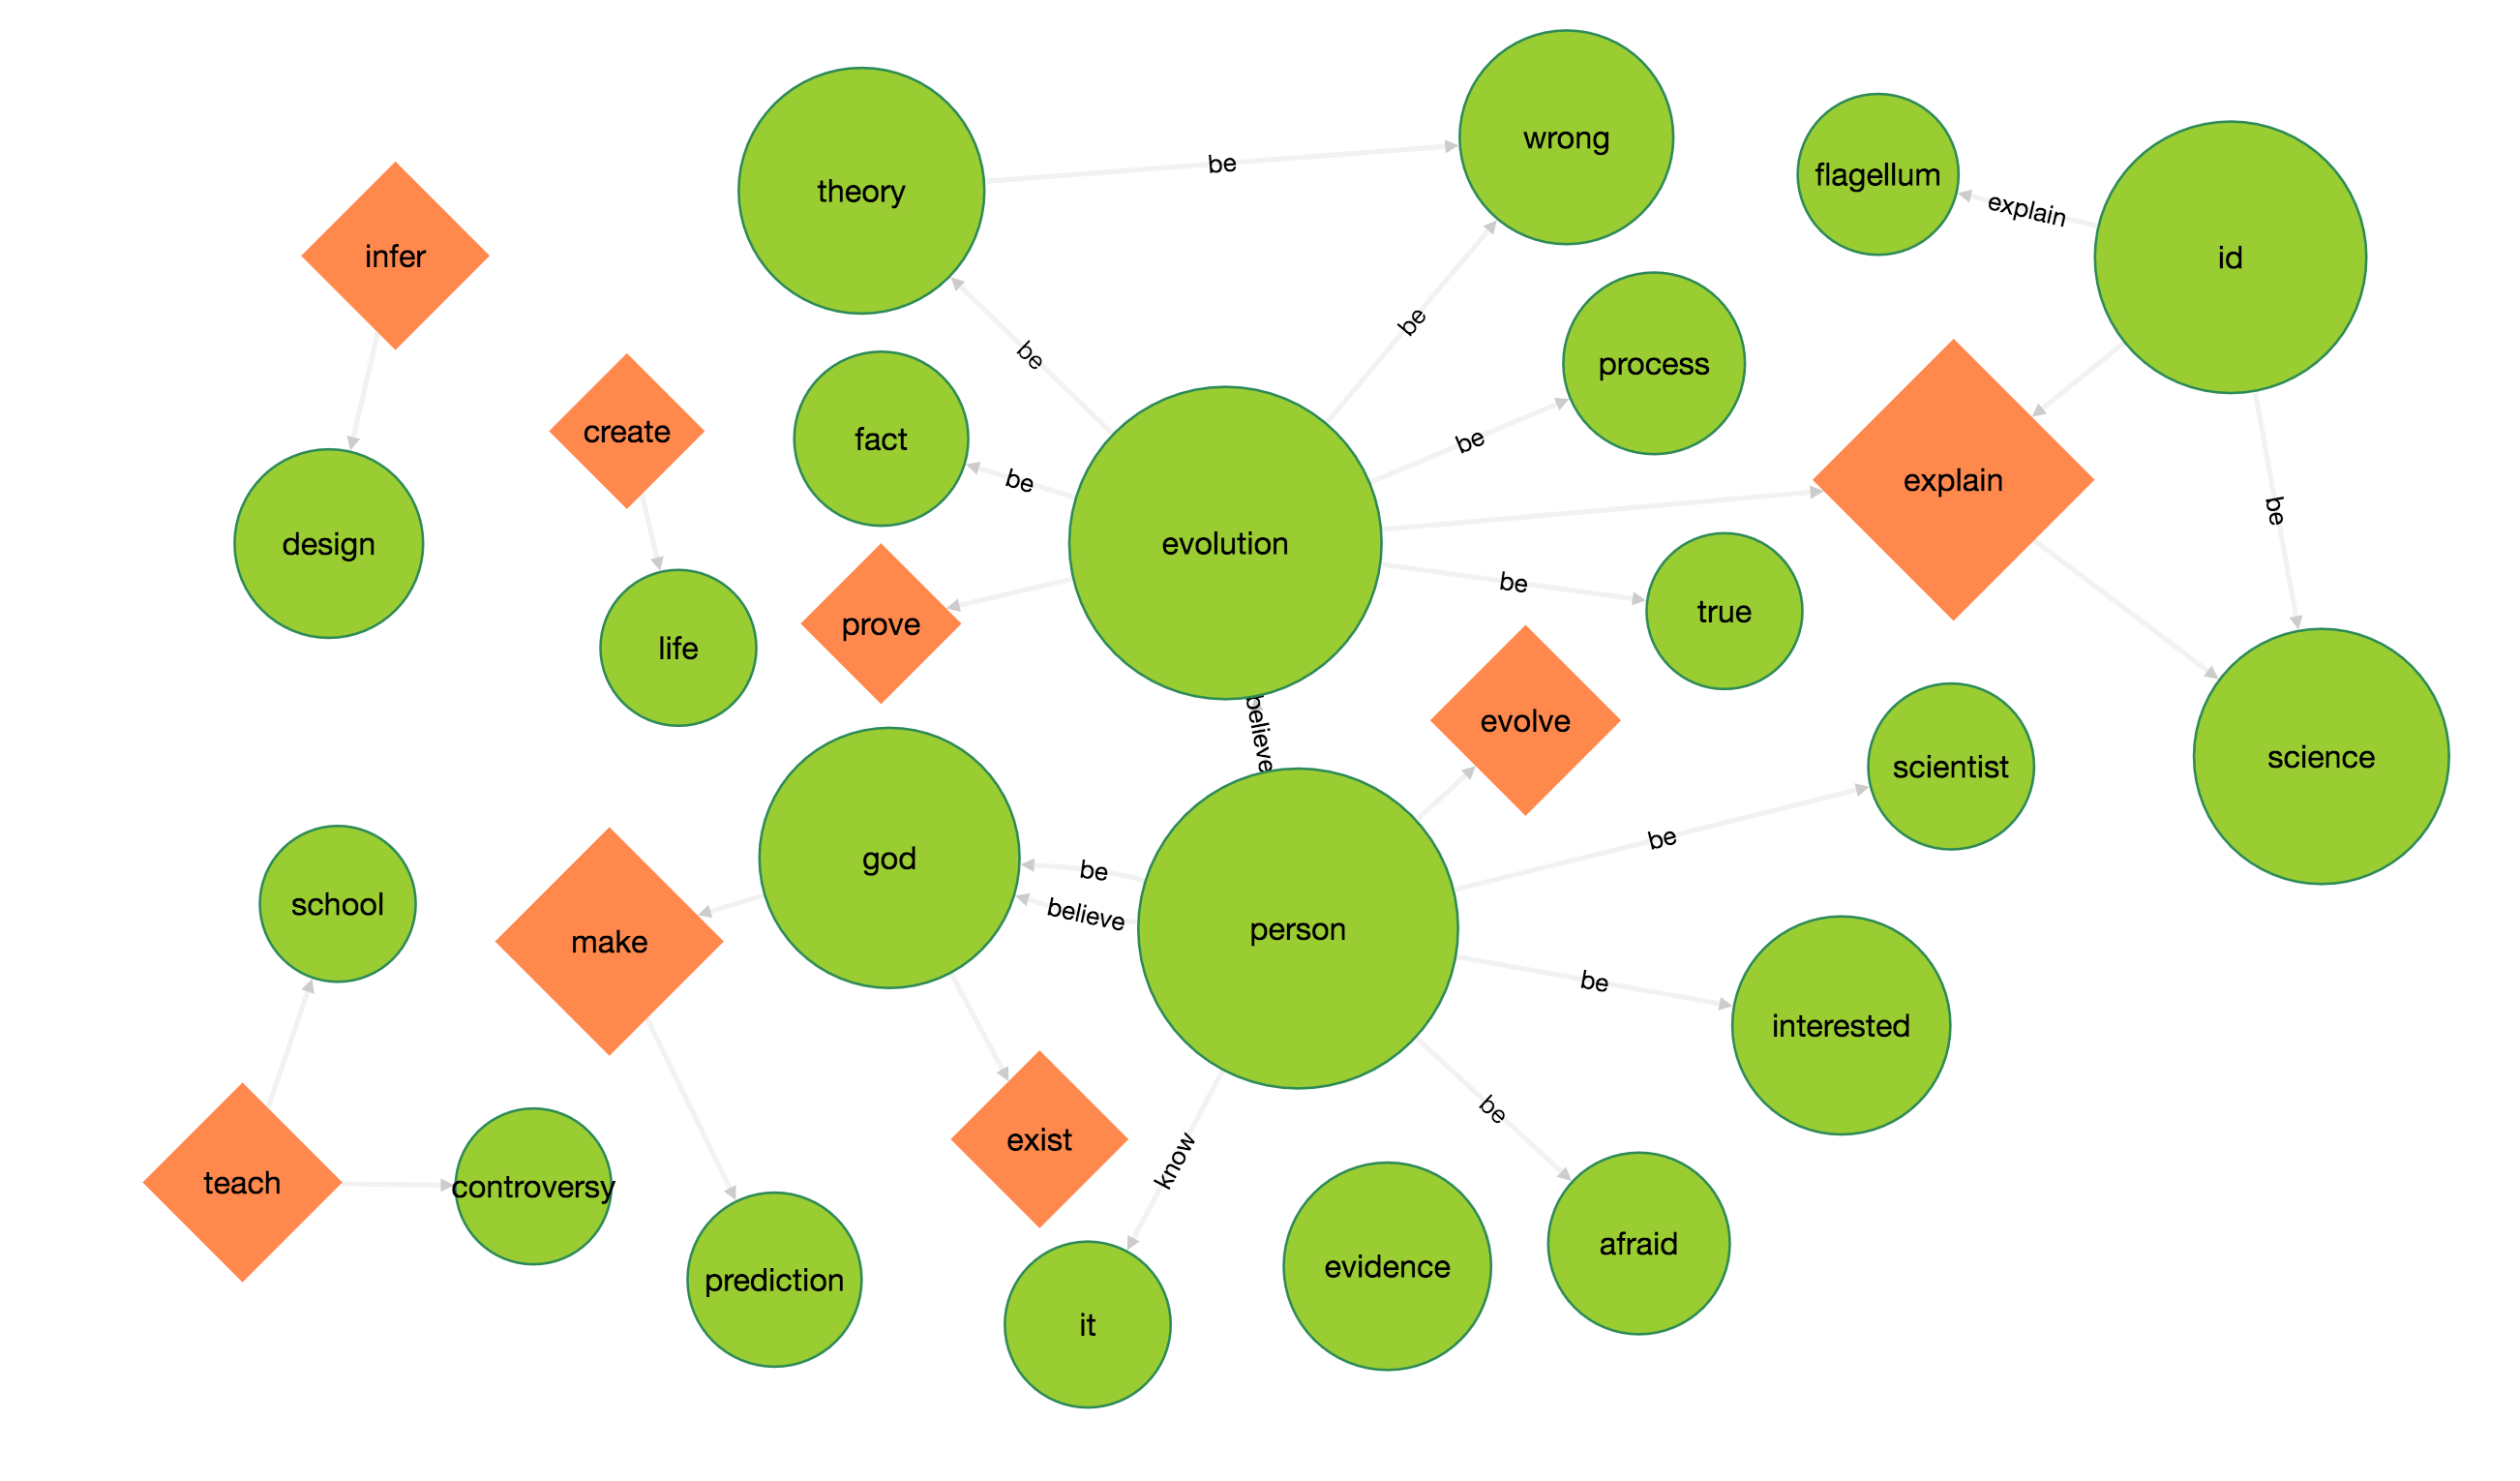
\includegraphics[width=0.45\textwidth]{disc_graph}}
      \fbox{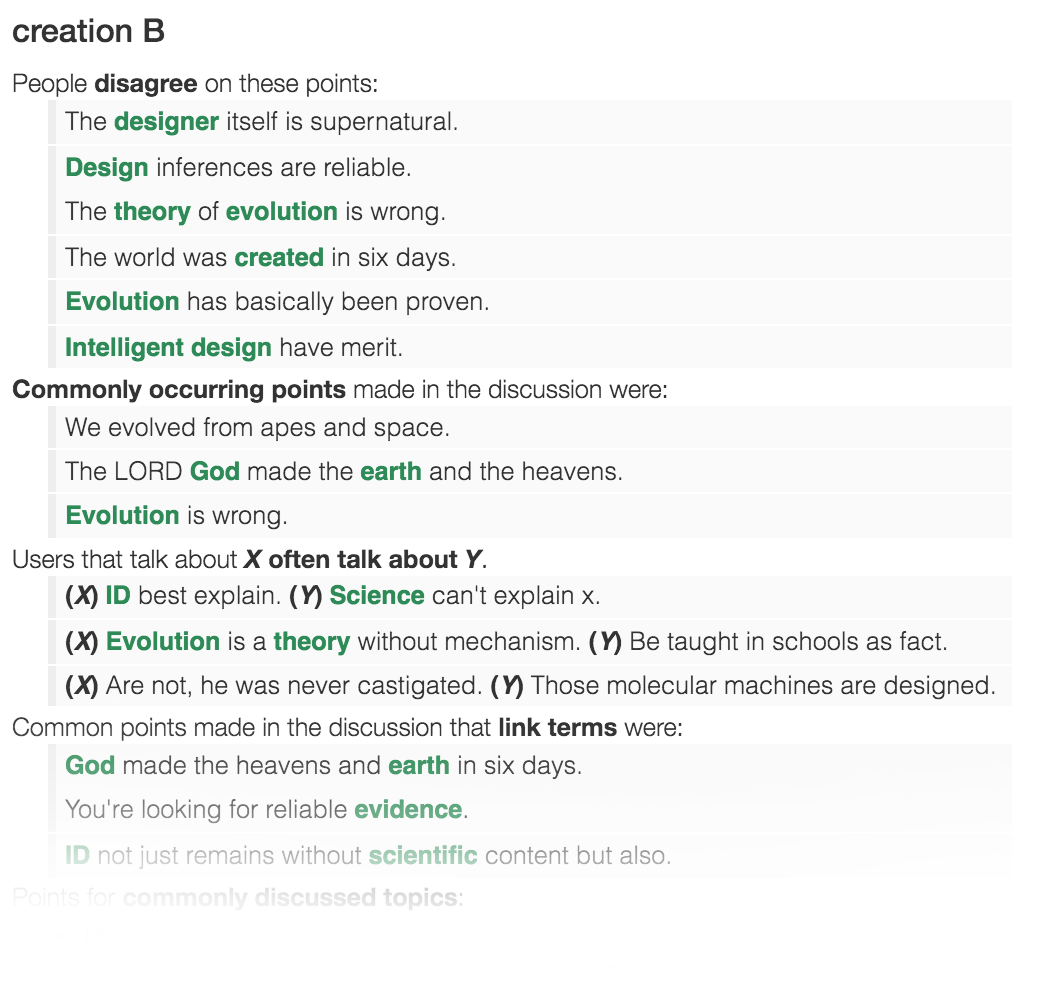
\includegraphics[width=0.45\textwidth]{summary}}

      What would be interesting to do next?

      \vfill
      \begin{center}
        \textbf{advaith@abdn.ac.uk} - \textbf{azwyner@abdn.ac.uk} -  \textbf{c@egan.co}
      \end{center}
    \end{center}
  \end{frame}

  {
	\usebackgroundtemplate{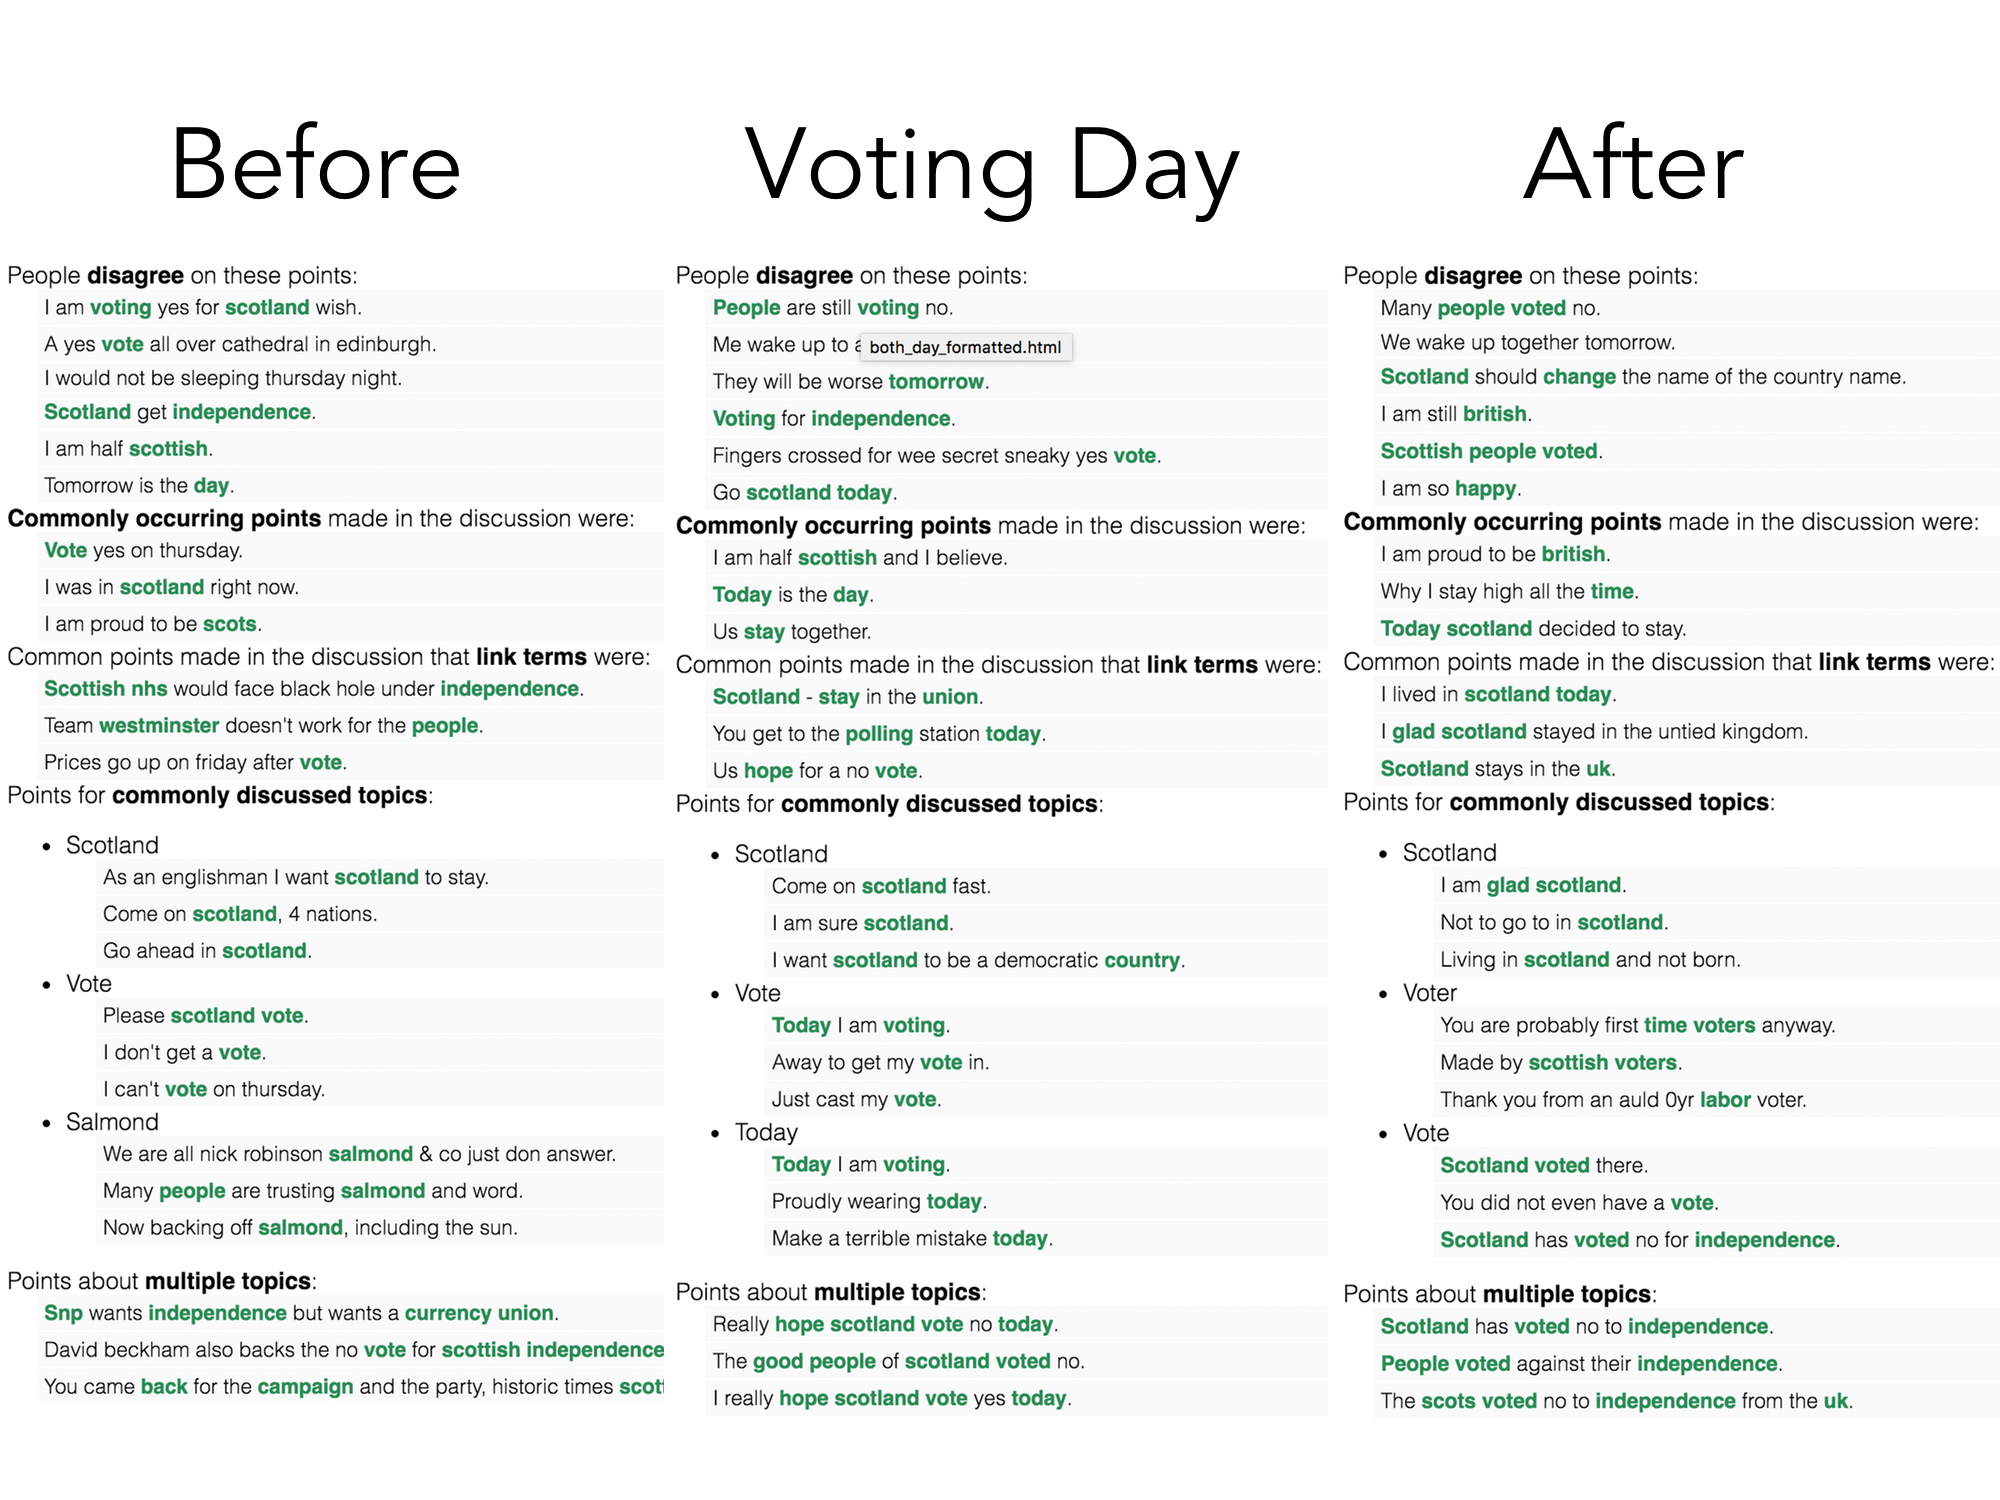
\includegraphics[height=\paperheight,width=\paperwidth]{compared}}
	\setbeamertemplate{navigation symbols}{}
	\begin{frame}[plain]
	\end{frame}
  }

  %\begin{frame}{Further Work
    %\begin{itemize}
      %\item{Web application interface}
      %\item{Adjustments for better performance on smaller sets of text}
      %\item{Improve means of selecting extracts}
      %\item{Add support for hierarchical conversations and Twitter replies}
      %\item{New presentations, e.g. connected graph structure}
      %\item{Greater focus on argumentation structures and semantics}
    %\end{itemize}
  %\end{frame}
\end{document}
